%%%%%%%% ICML 2021 EXAMPLE LATEX SUBMISSION FILE %%%%%%%%%%%%%%%%%

\documentclass{article}

% Recommended, but optional, packages for figures and better typesetting:
\usepackage{microtype}
\usepackage{graphicx}
\usepackage{subfigure}
\usepackage{booktabs} % for professional tables
\usepackage{placeins}
\usepackage{amsmath}
% \usepackage{subcaption}

% hyperref makes hyperlinks in the resulting PDF.
% If your build breaks (sometimes temporarily if a hyperlink spans a page)
% please comment out the following usepackage line and replace
% \usepackage{icml2021} with \usepackage[nohyperref]{icml2021} above.
\usepackage{hyperref}

% Attempt to make hyperref and algorithmic work together better:
\newcommand{\theHalgorithm}{\arabic{algorithm}}

% Use the following line for the initial blind version submitted for review:
\usepackage[accepted]{icml2021}



% If accepted, instead use the following line for the camera-ready submission:
%\usepackage[accepted]{icml2021}

% The \icmltitle you define below is probably too long as a header.
% Therefore, a short form for the running title is supplied here:
\icmltitlerunning{Sharpness Aware Transformers for Cost-Effective Image Classification}



\begin{document}

\twocolumn[
    % \icmltitle{Cost-Effective Model Configuration for Small Datasets in Image Classification}
    \icmltitle{Sharpness Aware Transformers for Cost-Effective Image Classification}

    \icmlsetsymbol{equal}{*}

    \begin{icmlauthorlist}
        \icmlauthor{Shreyansh Sharma S3772241}{equal,li}
    \end{icmlauthorlist}

    \icmlaffiliation{li}{Department of Computer Science, Leiden University, Leiden, Netherlands}

    \icmlcorrespondingauthor{Shreyansh Sharma}{s3772241@vuw.leidenuniv.nl}
    \vskip 0.3in
]
\printAffiliationsAndNotice{\icmlEqualContribution} % 

\begin{abstract}
    This paper presents a comparative analysis of pretrained image classification architectures for the CIFAR-100 dataset, with a focus on finding a novel configuration that performs well within smaller budgets and datasets. The study aims to identify an optimized model and its configuration that demonstrates superior performance compared to larger benchmarks like ImageNet, while considering resource constraints. The evaluated architectures include ResNets, Vision Transformers (VIT), and Swin Transformers. Additionally, different optimization techniques such as Adam and Adaptive Sharpness-Aware Minimization (ASAM) are examined to determine their impact on convergence and accuracy. The investigation incorporates the use of cosine annealing learning rate and step learning rate techniques for fine-tuning the training process.
    % By thoroughly comparing these architectures and optimization techniques, this research aims to identify a cost-effective and novel configuration for image classification tasks with smaller budgets and datasets.
\end{abstract}

\section{Introduction}
Image classification plays a crucial role in computer vision, enabling machines to understand and categorize visual content. With the rapid advancements in deep learning, various architectures have been developed to tackle image classification tasks. In this report, we compare four prominent architectures for image classification on the CIFAR-100 dataset \cite{Krizhevsky09learningmultiple}: Vision Transformer (VIT), Convolutional Vision Transformer (CVT), Swin Transformer, and Residual Networks (ResNets).

% While we compare different architectures, not all architectures are finetuned from scratch. We utilize existing open source models provided by others to have a baseline accuracy. 


In addition to the comparison of architectures, it is important to note that this report does not propose a new novel architecture for image classification. 
Instead, our focus lies in combining different optimizers and conducting extensive hyperparameter tuning to identify the best configuration specifically for the CIFAR-100 dataset, utilizing pretrained models.

Pretrained models have shown exceptional performance over the years in various image classification tasks. They are models that have been trained on large-scale datasets like ImageNet, which contain millions of images across numerous categories. 
By leveraging the knowledge and representations learned from these pretrained models, we aim to harness their transferability and apply them to the CIFAR-100 dataset.

% While the CIFAR-100 dataset has been widely used in the field of image classification, it is worth mentioning that not all previous works have thoroughly evaluated their proposed architectures, especially pretrained models, on this specific dataset.
% By conducting a comprehensive analysis on CIFAR-100 using pretrained models, we aim to bridge this gap and provide a fair and robust comparison.

% Change the para above to rephrase and talk about low budget

While pretrained models have been extensively used in image classification tasks, they are often evaluated on large-scale datasets like ImageNet. However, these models may not be suitable for smaller budgets and datasets, such as CIFAR-100. By conducting a thorough analysis of pretrained models on CIFAR-100, we aim to identify a cost-effective and novel configuration that performs well within smaller budgets and datasets.


Through the exploration of various optimizer algorithms and hyperparameter tuning techniques, we aim to find the optimal settings for each architecture, fine-tuning the pretrained models specifically for the CIFAR-100 dataset. 
This approach allows us to evaluate and compare the architectures on a level playing field, ensuring that the reported results reflect the true capabilities of the pretrained models in handling the complexities presented by CIFAR-100. 
By considering multiple aspects, including accuracy, computational requirements, and generalization abilities, we aim to provide valuable insights for practitioners and researchers in selecting the most suitable pretrained architecture for image classification tasks on CIFAR-100.

\section{Previous Work}
% Mention CNN
Significant progress has been made in image classification with the development of deep learning architectures. Traditional approaches primarily relied on convolutional neural networks (CNNs), such as the pioneering work of AlexNet (Krizhevsky et al., 2012). However, recent advancements have extended beyond CNNs to incorporate transformers, originally introduced for natural language processing tasks.

% mention resnet
Additionally, the Residual Networks (ResNets) proposed by He et al. (2015) have been widely adopted in image classification tasks. ResNets employ residual connections, enabling the construction of deep networks while mitigating the vanishing gradient problem. The skip connections in ResNets facilitate gradient flow during training, allowing for better convergence and improved performance.

% mention VIT and how its faster than CNN
One notable architecture is the Vision Transformer (VIT), proposed by Dosovitskiy et al. (2020). 
VIT revolutionized the field of image classification by leveraging self-attention mechanisms from transformers. 
By replacing traditional convolutional layers with self-attention mechanisms, VIT allows for global information exchange among pixels, enabling the model to capture long-range dependencies within images.
VIT has demonstrated impressive performance on large-scale datasets like ImageNet, showcasing its ability to learn meaningful representations from visual data. 
And additionally, VIT has shown to be more computationally efficient than CNNs, making it a valuable candidate for image classification tasks with limited resources.

% mention CVT
Building upon VIT, Wu et al. (2021) introduced the Convolutional Vision Transformer (CVT). 
CVT incorporates convolutional layers in conjunction with self-attention mechanisms to strike a balance between the efficiency of CNNs in capturing local image details and the expressive power of transformers in capturing global dependencies. 
This fusion of convolutional and transformer architectures shows promise in improving the overall performance of image classification models.

% mention SWIN
% REMOVE THIS PARAGRAPH IF IF DOESN'T FIT
Another recent architecture is the Swin Transformer proposed by Liu et al. (2021). 
Swin Transformer introduces hierarchical partitioning of image patches, allowing for efficient computation and capturing both local and global dependencies. 
By using shift windows, Swin Transformer reduces the computational complexity associated with traditional self-attention mechanisms, making it more scalable for larger image sizes.

% Finally, mention how these architectures are evaluated on CIFAR-100
By comparing these architectures on the CIFAR-100 dataset, we aim to evaluate their performance, computational requirements, and generalization capabilities for image classification tasks. 
This analysis will provide valuable insights into the strengths and weaknesses of each architecture, aiding researchers and practitioners in selecting appropriate models for image classification applications on a budget.
For the scope of this report, we do not experiment with CNN-based models, as they can be computationally expensive and require large amounts of data to train effectively.

\section{Dataset}
CIFAR-100 is a widely used benchmark dataset for image classification tasks. 
It consists of 60,000 color images in a 32x32 pixel resolution, belonging to 100 fine-grained object categories. 
The dataset is divided into training and testing sets, with 50,000 and 10,000 images respectively. 
Each image is labeled with one of the 100 classes, providing a challenging task for image classification algorithms due to the high level of intra-class variation.

CIFAR-100 has served as a valuable resource for evaluating and comparing various image classification algorithms and architectures. 
It has been extensively used in the literature to assess the performance and generalization capabilities of different approaches. 
Researchers often report classification accuracy, as well as other evaluation metrics, to demonstrate the effectiveness of their proposed methods on this dataset. 
The availability of a diverse range of object categories in CIFAR-100 enables comprehensive analysis and comparison of image classification models, facilitating advancements in the field.

% \section{Goal}

\section{Evaluation}
For the evaluation of the compared architectures, the top-1 accuracy metric is utilized. 
Top-1 accuracy measures the percentage of correctly predicted labels, considering only the most probable class prediction for each image. By focusing on the highest probability prediction, this metric provides a reliable measure of the models' classification performance. 
The top-1 accuracy is a widely used evaluation metric in image classification tasks as it reflects the model's ability to correctly identify the most dominant class for each image, thus providing insights into the effectiveness of the architectures in accurately classifying the CIFAR-100 dataset.

\section{Architectures}

\subsection{Resnet}
Residual Networks (ResNets) have emerged as one of the pioneering architectures in image classification tasks, demonstrating remarkable performance across various datasets. Introduced by \cite{he2016deep}, ResNets address the challenge of training deep neural networks by utilizing residual connections. These connections enable the network to bypass layers and pass information directly through skip connections, mitigating the vanishing gradient problem and facilitating the training of much deeper networks. ResNets have consistently achieved state-of-the-art results in large-scale datasets like ImageNet, making them a valuable candidate for evaluation on smaller budgets and datasets, such as CIFAR-100.

\subsection{VIT}
Vision Transformers (VIT) have revolutionized the field of image classification by introducing the power of transformers into computer vision tasks. Proposed by \cite{DBLP:journals/corr/abs-2010-11929}, VIT replaces the traditional convolutional layers with self-attention mechanisms, enabling the model to capture global dependencies among pixels. VITs have shown impressive performance on large-scale datasets like ImageNet, showcasing their ability to learn meaningful representations from visual data. Thus, evaluating VITs on smaller budgets and datasets, such as CIFAR-100, allows us to assess their effectiveness in leveraging self-attention mechanisms for image classification tasks with limited resources.

\begin{figure}[ht]
    \vskip 0.2in
    \centering
    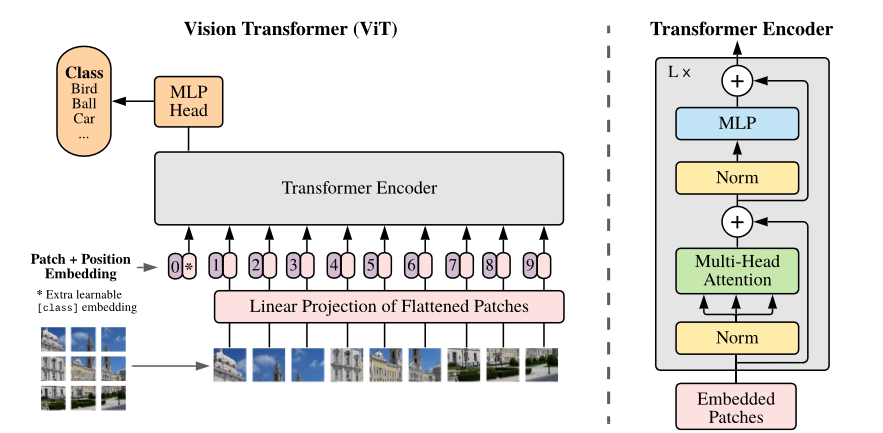
\includegraphics[width=0.4\textwidth]{vit.png}
    \caption{Illustration provided by \cite{DBLP:journals/corr/abs-2010-11929} represents the architecture of VIT}
    \label{fig:foobar}
    \vskip -0.2in
\end{figure}

\subsection{SWIN}
Swin Transformer, proposed by \cite{DBLP:journals/corr/abs-2103-14030}, is a novel architecture that introduces hierarchical partitioning of image patches, enabling efficient computation and capturing both local and global dependencies. By dividing the input image into non-overlapping patches, Swin Transformer incorporates shifted windows to reduce computational complexity compared to traditional self-attention mechanisms. Swin Transformer has shown impressive performance on large-scale image classification tasks, such as ImageNet, highlighting its ability to capture fine-grained details and long-range dependencies in images. Evaluating Swin Transformer on smaller budgets and datasets like CIFAR-100 allows us to assess its suitability for image classification tasks with limited resources.

\begin{figure}[ht]
    \vskip 0.2in
    \centering
    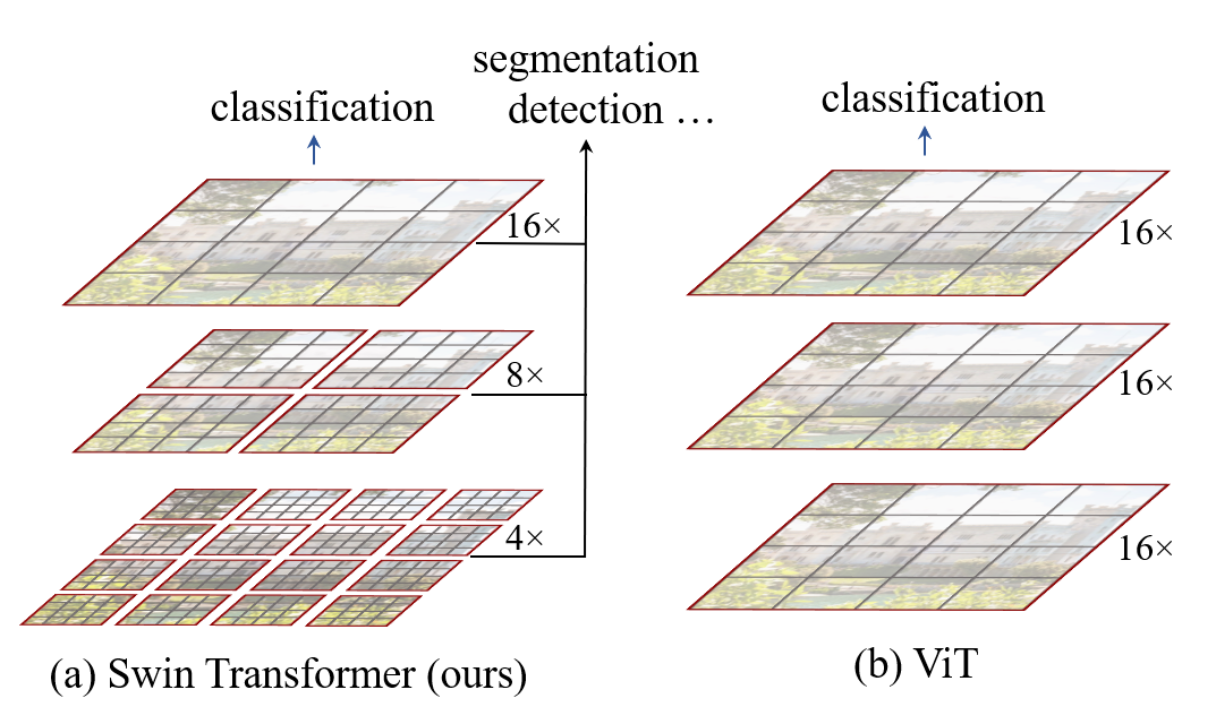
\includegraphics[width=0.4\textwidth]{swin.png}
    \caption{Illustration provided by \cite{DBLP:journals/corr/abs-2103-14030} represents how SWIN architecture is different from VIT.}
    \label{fig:foobar}
    \vskip -0.2in
\end{figure}

\section{Hyperparameter tuning}
All models that were trained for the experiments were pretrained models which needed to be finetuned in order to evaluate on CIFAR-100. So no parameters specific to the network architecture were tuned. For decreasing the number of epochs to achieve higher accuracies we experimented with optimizers and learning rate schedulers.

\begin{table}[ht]
    \centering
    \begin{tabular}{|l|l|}
        \hline
        \multicolumn{2}{|c|}{\textbf{Hyperparameters}} \\ \hline
        lr            & 1e-2                           \\ \hline
        gamma         & 0.95                           \\ \hline
        step\_size    & 100                            \\ \hline
        optimizer     & ASAM                           \\ \hline
        batch\_size   & 32                             \\ \hline
        lr\_scheduler & Step                           \\ \hline
        epochs        & 5                              \\ \hline
        momentum      & 0.9
        \\ \hline
    \end{tabular}
    \caption{Hyperparameters that were selected after running multiple iterations.}
    \label{tab:actor_critic_hp}
\end{table}

\subsection{Optimizer}

\subsubsection{Adam}
Adam (Adaptive Moment Estimation) is an optimization algorithm commonly used in deep learning for training neural networks. 
Introduced by \cite{Kingma2014AdamAM}, Adam combines the advantages of adaptive learning rates and momentum-based optimization. 
It maintains adaptive learning rates for each parameter by utilizing estimations of both first-order moments (the mean) and second-order moments (the uncentered variance) of the gradients. 
By incorporating momentum, Adam effectively handles sparse gradients and accelerates convergence. 
For the experiments on ADAM we utilized models that were already finetuned on CIFAR-100 for VIT, SWIN, and Resnet model architectures.

\subsubsection{ASAM}
Adaptive Sharpness-Aware Minimization (ASAM) is an optimization algorithm introduced by \cite{DBLP:journals/corr/abs-2102-11600} to enhance gradient-based optimization in deep learning. 
SAM adapts the learning rate for each parameter based on the sharpness of the loss landscape, allowing for more precise optimization and improved generalization. 
By modulating the learning rates using sharpness estimates, SAM aims to mitigate the issue of being trapped in suboptimal sharp minima.

SAM offers a potential advantage over Adam by addressing the issue of suboptimal sharp minima in deep learning optimization. 
While Adam performs well in many scenarios, it can struggle when faced with sharp minima, potentially leading to less optimal solutions. 
In contrast, SAM's adaptivity to the sharpness of the loss landscape allows it to modulate learning rates accordingly, potentially leading to better generalization and avoiding convergence in suboptimal sharp minima. 
Evaluating SAM alongside Adam on different architectures, such as Vision Transformers and Swin Transformers for CIFAR-100 classification tasks provides an opportunity to assess whether SAM's sharpness-aware optimization can yield improved results and potentially outperform Adam in terms of convergence, accuracy, and robustness.

From \textit{Figure 3} we can see that VIT-ASAM converges faster than VIT-ADAM. 
These results can be considered biased as the goal of the hyperparameter tuning was to find optimal paramteters for modeling with ASAM instead of ADAM and lesser exploration was done in order achieve better results from ADAM.


\begin{figure}[ht]
    \vskip 0.2in
    \centering
    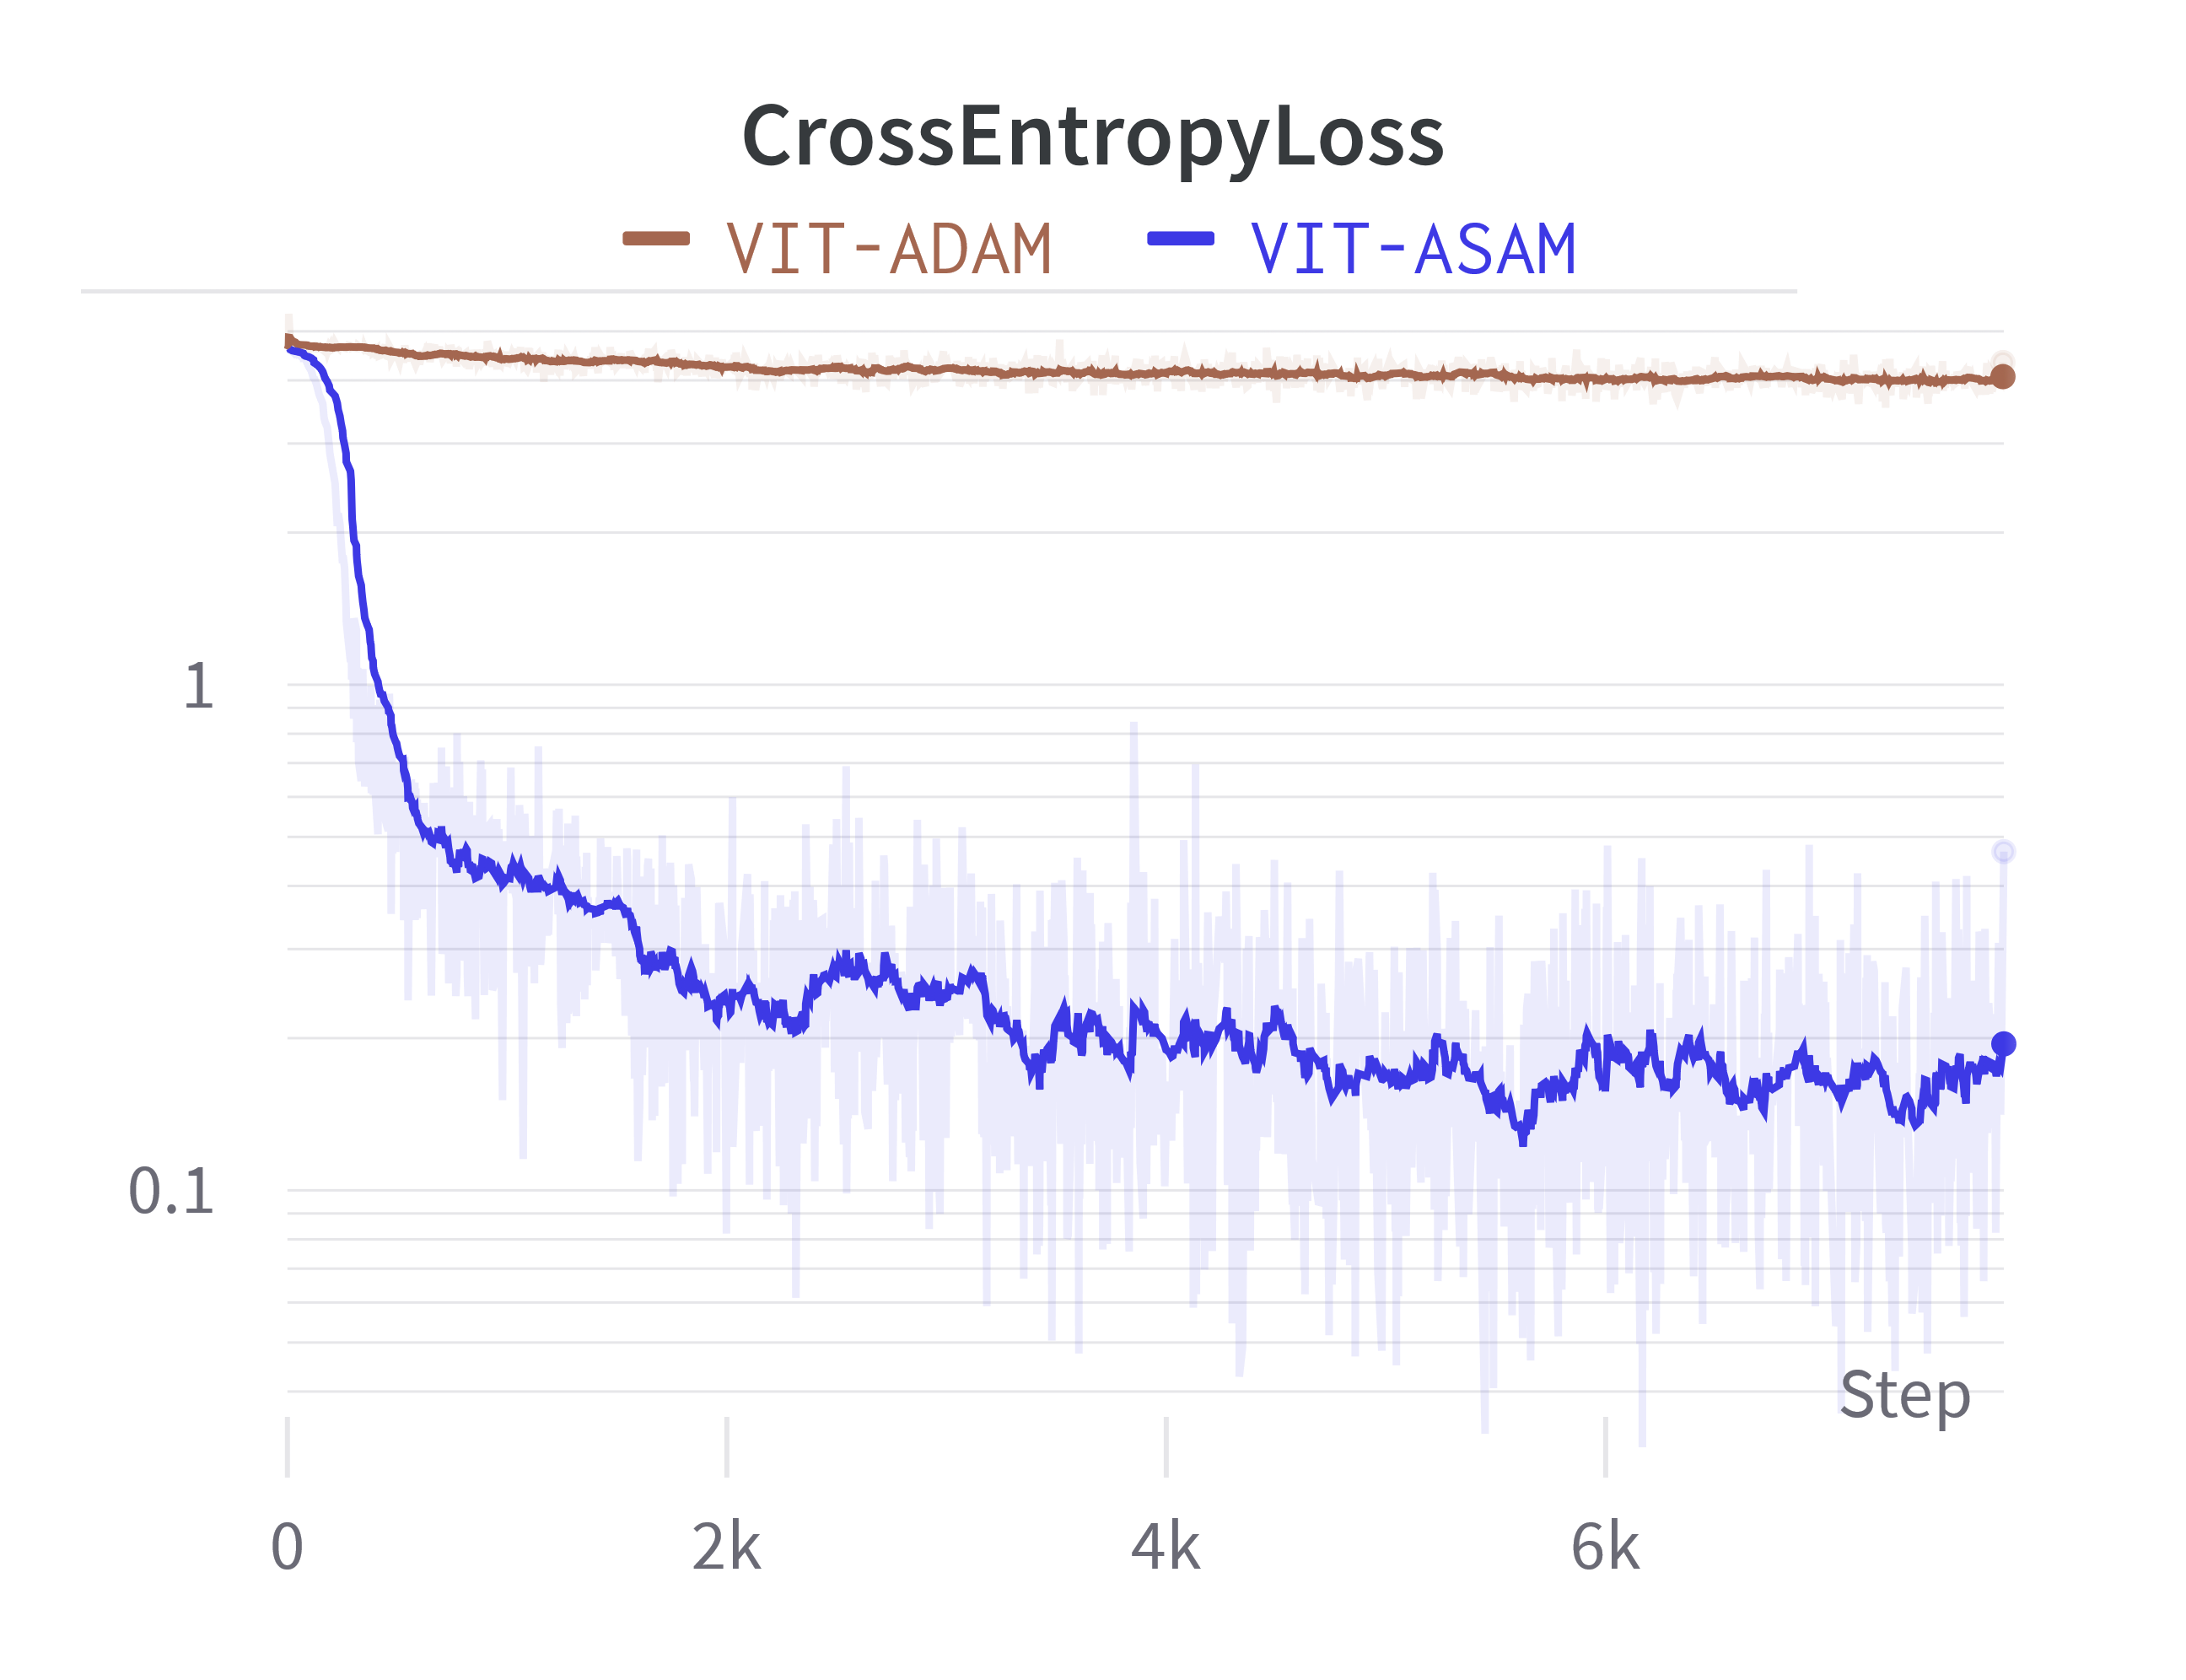
\includegraphics[width=0.4\textwidth]{optimizers.png}
    \caption{Comparing our selected hyperparameters for VIT-ADAM and VIT-ASAM. This result itself is biased since VIT-ADAM pretrained already existed the goal of hyperparameter tuning was to find the best parameters for ASAM.}
    \label{fig:foobar}
    \vskip -0.2in
\end{figure}

\subsection{Schedulers}
\subsubsection{Cosine Annealing LR}
Cosine annealing learning rate (CLR) is a technique commonly used in image classification to optimize the learning rate schedule. 
By gradually reducing the learning rate following a cosine-shaped curve, CLR improves convergence, helps avoid overfitting, and enhances generalization. 
It allows the model to take larger steps initially, exploring a wider parameter space, and then fine-tune its parameters as training progresses. 
CLR has been successfully applied to various architectures like ResNets, Vision Transformers, and Swin Transformers, leading to improved accuracy and better generalization on datasets such as CIFAR-100. 
Overall, CLR is an effective strategy for optimizing learning rates in image classification, contributing to improved performance and model robustness.


\subsubsection{Step LR}
Step learning rate (StepLR) is a popular strategy used in image classification to adjust the learning rate during training. 
With StepLR, the learning rate is reduced by a fixed factor at predetermined steps or epochs. 
Fine-tuning the StepLR schedule by carefully selecting the step size and reduction factor can lead to improved results in image classification tasks. 
By gradually decreasing the learning rate at specific intervals, StepLR allows the model to converge more effectively and find better optima. 
This fine-tuning process helps to stabilize the training process, prevent overfitting, and achieve higher accuracy on various datasets, making it a valuable technique for optimizing the learning rate schedule in image classification.

% compare step lr and cosine annealing lr
From \textit{Figure 4} we can see that Step LR converges faster than Cosine Annealing LR. 
This is because the learning rate is reduced by a fixed factor at predetermined steps or epochs. 
This helps to stabilize the training process, prevent overfitting, and achieve higher accuracy on various datasets, making it a valuable technique for optimizing the learning rate schedule in image classification.

\begin{figure}[ht]
    \vskip 0.2in
    \centering
    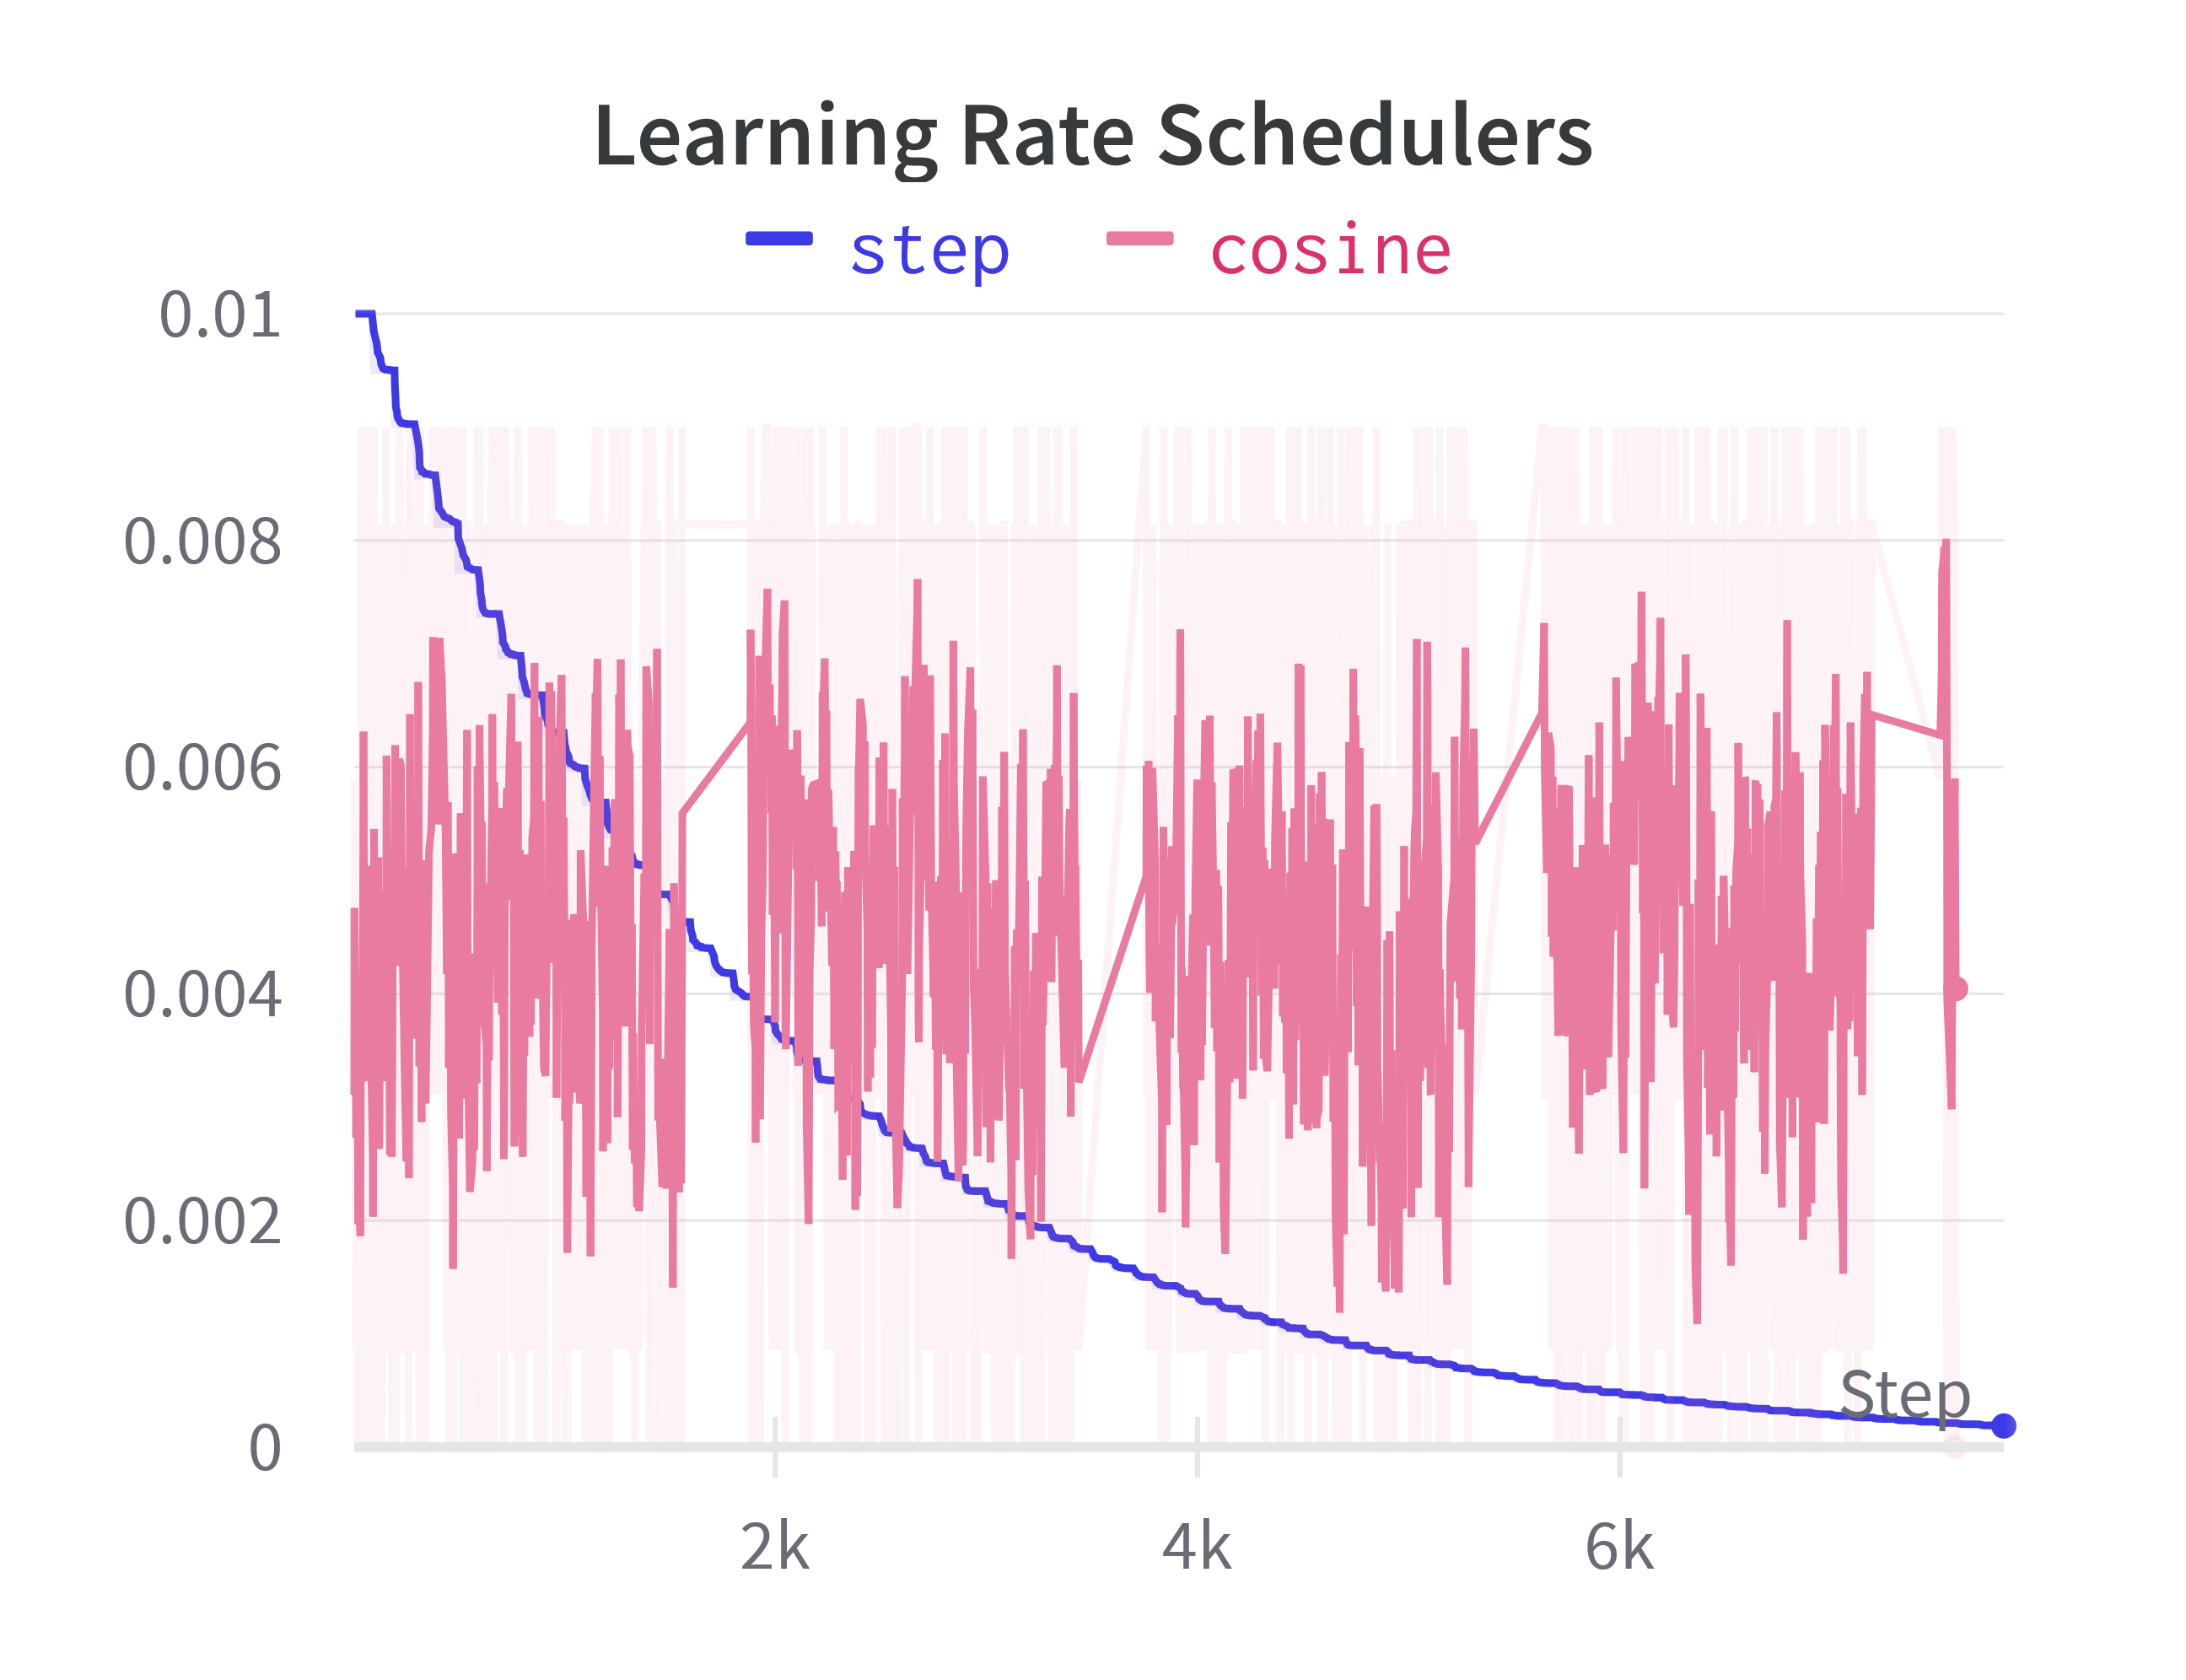
\includegraphics[width=0.4\textwidth]{learning_rate_schedulers.png}
    \caption{A visualization of how a Cosine Annealing LR works compared to a Step annealing LR scheduler}
    \label{fig:foobar}
    \vskip -0.2in
\end{figure}


\section{Experiments}
In order to find cost-effective model configurations for CIFAR-100 dataset, the epochs were set to a maximum of 5. 
This was chosen based on current SOTA models usually having an average range of 5-20 epochs over a pretrained model. 
Then for the optimizer we chose ASAM as our primary optimizer as it reduces the loss value faster than ADAM and converges to the optima. 
Additionally from our hyperparameter tuning excercise we found both Cosine Annealing and Step LR to give good accuracies, but since we needed a faster convergence we decided to choose Step LR for it's lower variance.

% compare vit and swin on ASAM with selected hyperparameters
\subsection{VIT VS SWIN}
VIT-ASAM is the model pretrained on imagenet21k and then finetuned on CIFAR-100 using ASAM and selected hyperparameters as shown in \textit{Table 1}. 
And on thee other hand SWIN-ASAM-frozen is the model pretrained on imagenet1k and finetuned using the same hyperparameters.

The reason to finetune SWIN with frozen weights was that it didn't converge fast enough under 5 epochs with the same hyperparameters and additionally with the same hardware specifications the batch size needed to be reduced due to low GPU memory. 
Hence it was decided to freeze the weights of the SWIN model architecture.

Looking at \textit{Figure 5} and \textit{Figure 6} we can see that VIT-ASAM outperforms SWIN-ASAM-frozen and gives a higher Top-1 accuracy of 92.85\% whereas SWIN-ASAM-frozen gives an accuracy of 92.023\%. 
Also it can be seen that SWIN performs better over the 1st epoch and over time diverges from the optima. 
Similar behaviour can be seen in \textit{Table 2} which showcases VIT outperforming SWIN for CIFAR-100 on the avaialable pretrained models. 
Finally, we can see that both the architectures show high standard deviation error which can be attributed to the small dataset size of CIFAR-100.

\begin{figure}[ht]
    \vskip 0.2in
    \centering
    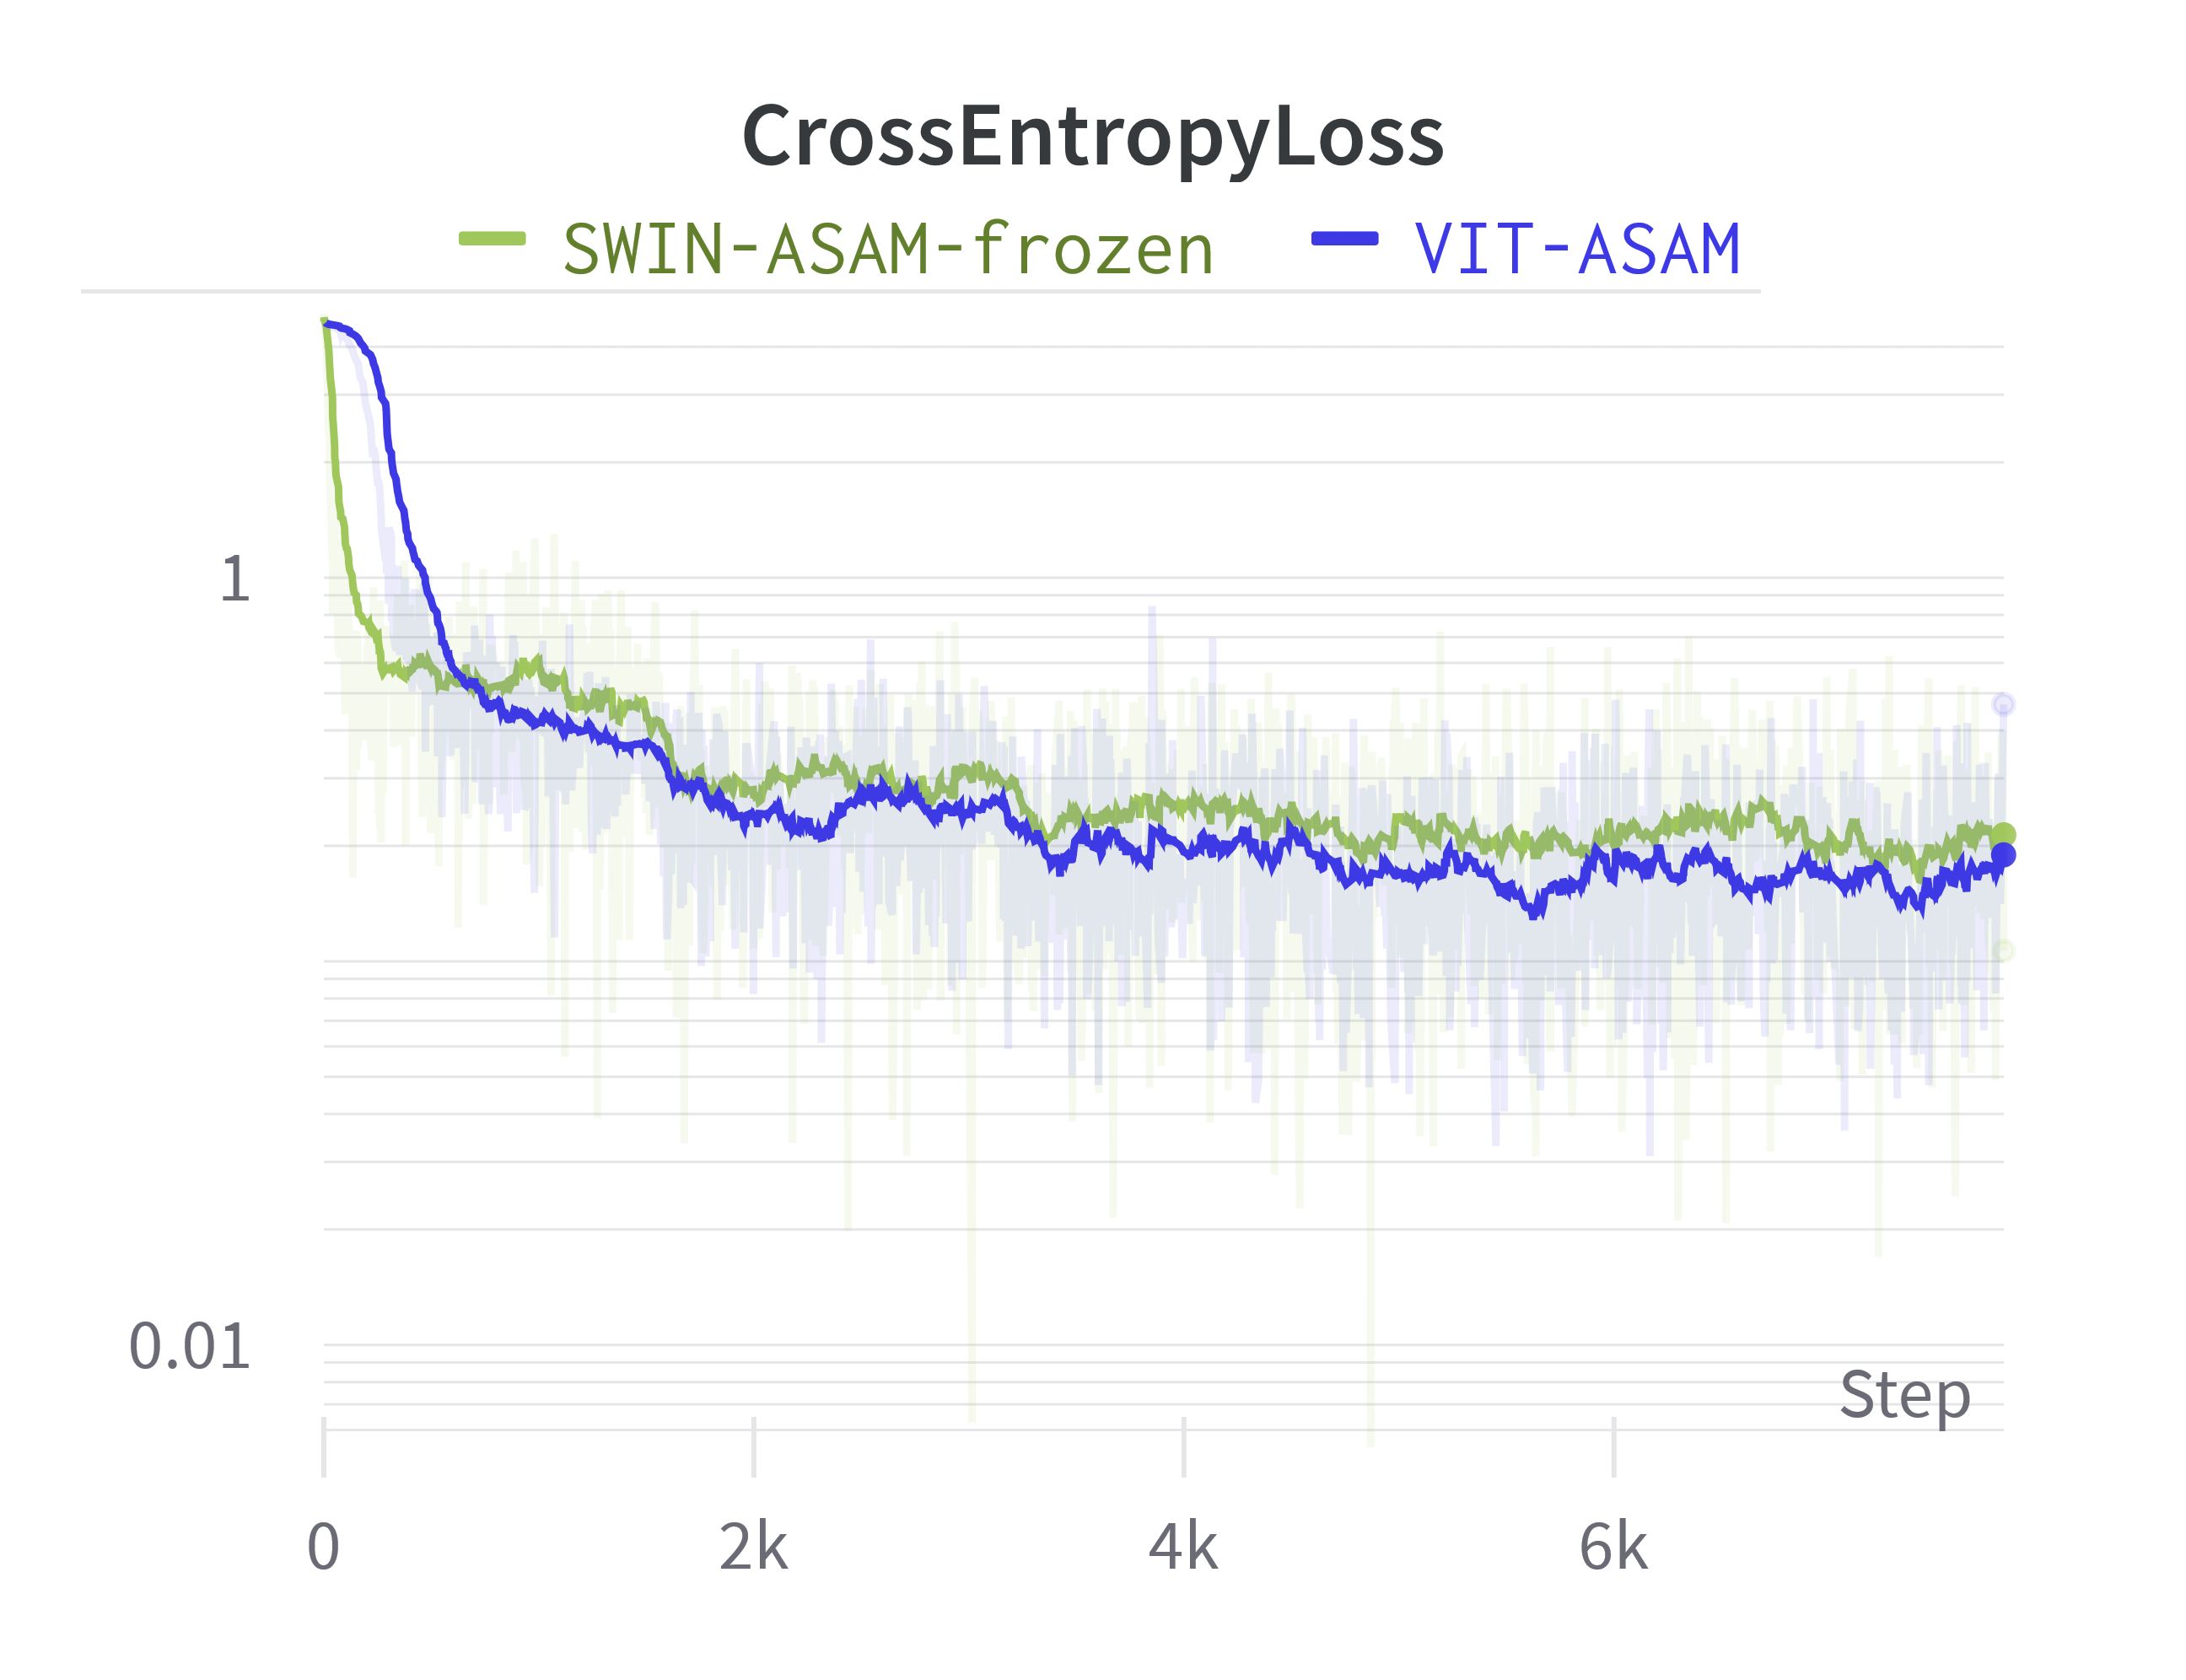
\includegraphics[width=0.4\textwidth]{cross_entropy_loss.png}
    \caption{Visualization of loss decreasing over steps for VIT-ASAM and SWIN-ASAM-frozen. WE can see that VIT-ASAM has a lower loss value after 5 epochs.}
    \label{fig:foobar}
    \vskip -0.2in
\end{figure}

\begin{figure}[ht]
    \vskip 0.2in
    \centering
    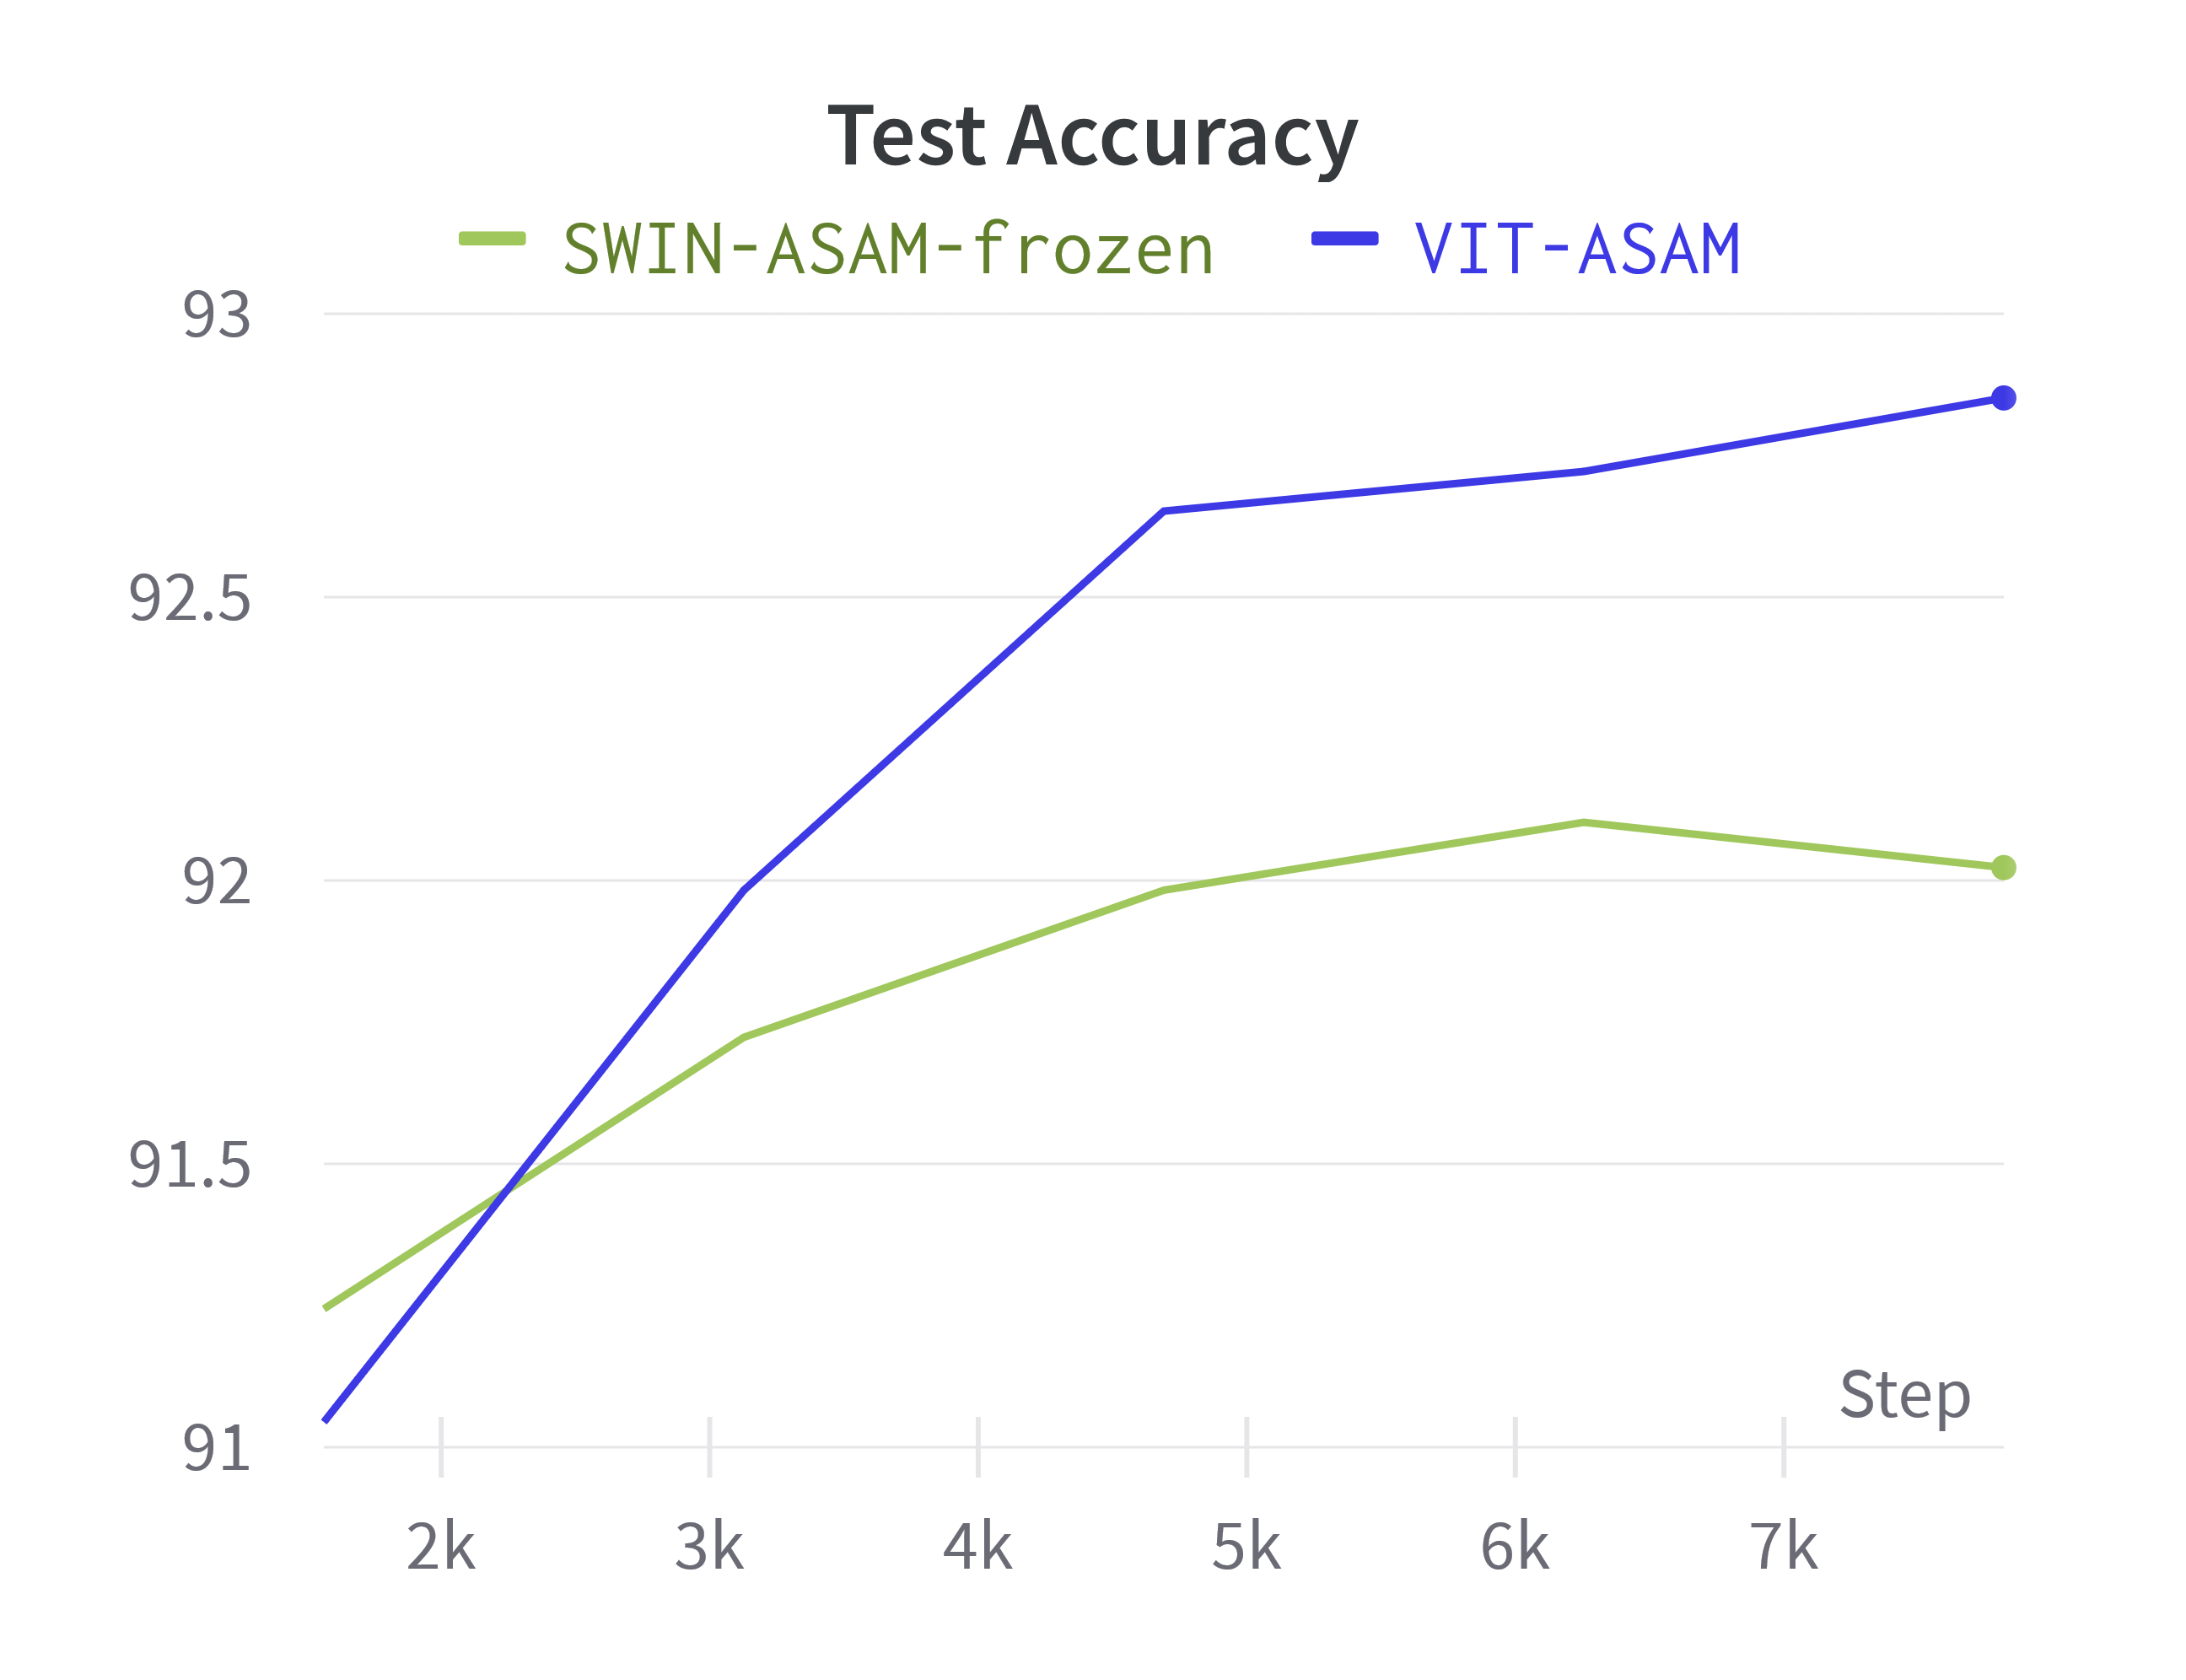
\includegraphics[width=0.4\textwidth]{test_accuracy.png}
    \caption{Visualization of loss decreasing over steps for VIT-ASAM and SWIN-ASAM-frozen. We can see that VIT-ASAM has a lower loss value after 5 epochs and converges to the optima.}
    \label{fig:foobar}
    \vskip -0.2in
\end{figure}

\section{Results \& Discussion}
From the experiments we were able to train 2 architectures which showcased high accuracies after intensive hyperparameter tuning and finetuning. 
In this section we will compare the achieved accuracies with the pretrained models which are considered SOTA for CIFAR-100. 
Only models that could be evaluated during our experiments are reported, although there exist SOTA models for which pretrained weights aren't available.

From \textit{Table 2} we can see that VIT-ASAM outperforms all other benchmarks with an accuracy of 92.851\%, that were evaluated against it. 
SWIN-ASAM also performs much better than it's ADAM variant with an accuracy of 92.023\% and converges to high accuracies within 5 epochs.

% fix resnet eval and talk about it
Resnet pretrained model was evaluated on CIFAR-100 and it gives an accuracy of 72.63\% which is much lower than the other models.
This can be attributed to the fact that Resnet pretrained weights are not readily available for CIFAR-100 and hence the model was used from open source implementations and might not reflect the true performance of the model.

\begin{table}[ht]
    \begin{tabular}{|l|l|c|l|}
        \hline
        \textbf{Model} & \textbf{Epochs} & \textbf{Loss} & \textbf{Top-1 Accuracy} \\ \hline
        Resnet         & 200             & 0.0284        & 72.63                   \\ \hline
        VIT            & 4               & 0.0402        & 89.85                   \\ \hline
        SWIN           & 14              & 0.0102        & 89.38                   \\ \hline
        VIT-ASAM       & 5               & 0.1411        & \textbf{92.851}         \\ \hline
        SWIN-ASAM      & 5               & 0.1208        & 92.023                  \\ \hline
    \end{tabular}
    \caption{Results for pretrained models and finetuned models for CIFAR-100}
\end{table}


\section{Conclusion and Future Work}
To sum up, we have compared various model architectures on CIFAR-100 dataset.
%  write the previous line better 
Not all SOTA models/algorithms were implemented due to unavailabilioty of pretrained weigjts and limited computational power. 
Since the scope of the report was to find cost-effective model configurations CNN architectures were not considered, as previous works have shown that they are computationally expensive.

From the experiments we can conclude that VIT-ASAM performs the best for CIFAR-100 dataset with an accuracy of 92.851\% and SWIN-ASAM is the second best model with an accuracy of 92.023\%.
Additionally, we can conclude that ASAM performs better than ADAM for smaller number of epochs and converges to the optima faster.

Since VIT-ASAM outperforms all other models, for future work we can try to finetune the model for more epochs and see if it can achieve higher accuracies.
Also hyperparameter tuning can be a time taking process and we can try to automate it using AutoML or Evolutionary Algorithms.

To the best of our knowledge, this is the first work that incorporates ASAM for transformer based architectures on CIFAR-100 dataset.
This report was inspired by the work of \cite{DBLP:journals/corr/abs-2102-11600} and \cite{DBLP:journals/corr/abs-2103-14030} and we hope that this report can be used as a reference for future works.


% In the unusual situation where you want a paper to appear in the
% references without citing it in the main text, use \nocite
\nocite{*}


\bibliography{main.bib}
\bibliographystyle{icml2021}

\end{document}